%!TEX TS-program = xelatex
%!TEX encoding = UTF-8 Unicode

\documentclass[11pt,tikz,border=1]{standalone}
\usetikzlibrary{circuits.logic.US,positioning,decorations.pathreplacing,math}

\begin{document}
  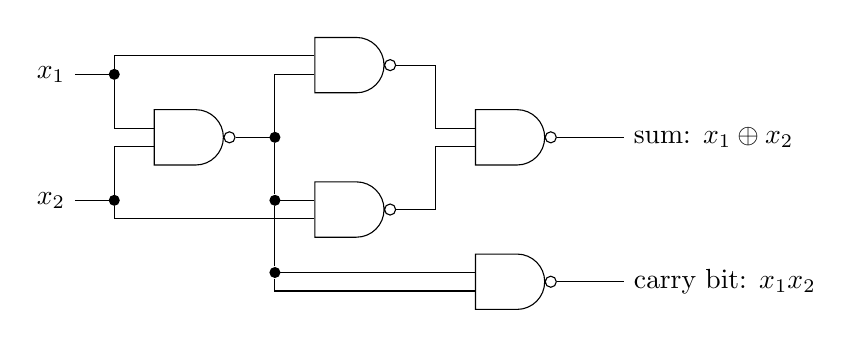
\begin{tikzpicture}[
    circuit logic US, large circuit symbols,
    contact/.style={circle, fill=black, minimum size=4pt, inner sep=0pt}
    ]

    \matrix [column sep=1cm,row sep=2mm] {
                                 & \node [nand gate] (n1) {}; &                               \\
      \node [nand gate] (n2) {}; &                            & \node [nand gate] (sum) {};   \\
                                 & \node [nand gate] (n3) {}; &                               \\
                                 &                            & \node [nand gate] (carry) {}; \\
    };

    \node (x1) [left=of n2,yshift=8mm] {$x_1$};
    \node (x2) [left=of n2,yshift=-8mm] {$x_2$};
    \node (text1) [right=of sum] {sum: $x_1 \oplus x_2$};
    \node (text2) [right=of carry] {carry bit: $x_1x_2$};

    % connections:
    \draw (x1.east) -- ++(right:5mm) node [contact] (x1split) {} |- (n1.input 1);
    \draw (x1split) |- (n2.input 1);

    \draw (x2.east) -- ++(right:5mm) node [contact] (x2split) {} |- (n2.input 2);
    \draw (x2split) |- (n3.input 2);

    \draw (n2.output) -- ++(right:5mm) node [contact] (split1) [] {} |- (n1.input 2);
    \draw (split1 |- n3.input 1) node[contact] (split2) {} -- (n3.input 1);
    \draw (split2 |- carry.input 1) node[contact] (split3) {} -- (carry.input 1);

    \draw (split1) -- (split2) -- (split3) |- (carry.input 2);

    \draw (n1.output) -- ++(right:5mm) |- (sum.input 1);
    \draw (n3.output) -- ++(right:5mm) |- (sum.input 2);

    \draw (sum.output) -- (text1.west);
    \draw (carry.output) -- (text2.west);

  \end{tikzpicture}
\end{document}
